\documentclass[12pt,a4paper]{report}
\usepackage[utf8]{inputenc}
\usepackage[brazilian]{babel}
\usepackage{amsmath}
\usepackage{amsfonts}
\usepackage{amssymb}
\usepackage{graphicx}
\usepackage[table]{xcolor}
%\usepackage{breakcites}
%\usepackage{subfigure}
\usepackage{hyperref}
%pacote para escrever algoritmos
%http://www.cs.toronto.edu/~frank/Useful/algorithm2e.pdf
\usepackage[lined, boxed, portuguese, commentsnumbered]{algorithm2e}

\author{
  Bramigk, Victor\\
  \texttt{victorbramigk@gmail.com}
  \and
  Segre, Jan\\
  \texttt{jan@segre.in}
}
\title{Análise de logs de jogos da SSL (Robocup)}

\renewcommand*\thesection{\arabic{section}}
%\linespread{1.5}

\begin{document}
% capas obrigatorias
\begin{center}
\textbf{MINISTÉRIO DA DEFESA}\\
\textbf{EXÉRCITO BRASILEIRO}\\
\textbf{DEPARTAMENTO DE CIÊNCIA E TECNOLOGIA}\\
\textbf{INSTITUTO MILITAR DE ENGENHARIA}\\
\textbf{Seção de Engenharia de Sistemas / SE 8}

\vspace{2.5cm}

\begin{large}
\textbf{Proposta de Tema de Dissertação de Mestrado
\\Curso: Mestrado em Sistemas e Computação}

\vspace{1.5cm}

\textbf{Sistema de Localização de Objetos para Apoio a um Assistente Robótico Móvel na Casa Inteligente}

\vspace{1.5cm}

\textbf{Aluno: Fulano}

\vspace{1.5cm}

\textbf{Orientador: Paulo F. F. Rosa, Ph.D}

\end{large}

\vspace{2cm}

\begin{small}
Data de Apresentação no SE/8:\\
Rio de Janeiro, \today
\end{small}

\end{center}

\pagebreak

\newpage

\begin{large}
\chapter*{Título da Dissertação}

\textbf{Título da Tese:}
\bigskip

\textbf{Sistema de Localização de Objetos para Apoio a um Assistente Robótico Móvel na Casa Inteligente}

\bigskip
\noindent\textbf{Título da Capa:}
\bigskip

\textbf{Sistema de Localização de Objetos para Apoio a um Assistente Robótico Móvel na Casa Inteligente}

\bigskip
\noindent\textbf{Área de Concentração:}
\bigskip

Tecnologias e Sistemas de Computação

\bigskip
\noindent\textbf{Linha de Pesquisa:}
\bigskip

Tecnologias para Tratamento e Transmissão da Informação
\end{large}

\tableofcontents

\pagebreak


% resumo
\chapter*{Resumo}

O objetivo deste trabalho é prever como um time de futebol de robôs irá se comportar baseado
somente nas posições e orientações de um conjunto discreto de amostras. Para isso, foram estudados
os métodos da ACO (Ant Colony Optimization), SA (Simulated Annealing), Algorítimo  Genético, Lógica Nebulosa
e Redes Neurais. A partir do estudo detalhado desse algoritmos definiu-se duas linhas principais de
ação para a solução do problema: uma baseada em Logica Nebulosa e a outra baseada em Redes Neurais. Após
um estudo mais aprofundado deseja-se implementar um processo de otimização em ambos os algorítimos para
que o resultado seja refinado.


% introdução

% modelos
\frame{
  \frametitle{Lógica Nebulosa}
  \begin{block}{}
    \begin{figure}
      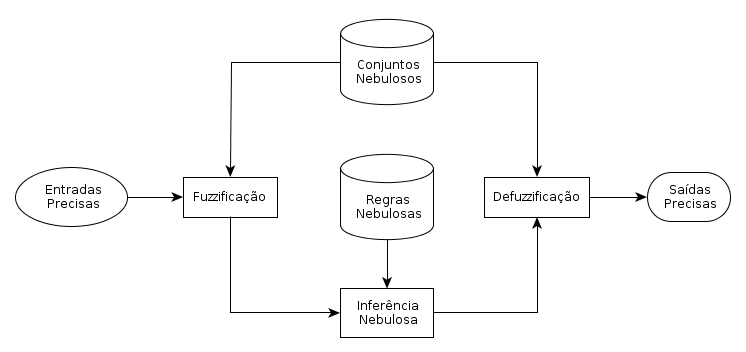
\includegraphics[width=0.8 \linewidth]
      {imgs/arquitetura_fuzzy}
      \caption{Arquitetura Funcional Genérica de um Sistema
      Nebuloso}
    \end{figure}
  \end{block}
}

\frame{
  \frametitle{Lógica Nebulosa}
  \begin{block}{}
    \textbf{Exemplo} Determinar o valor da apólice de seguro
    a ser paga pelo cliente João, cuja idade é 35 anos e a
    pressão arterial é de (130,75). As regras são:
    \begin{itemize}
      \item \emph{SE} idade é \textit{meia-idade} \emph{E}
            pressão arterial é \textit{baixa} \emph{ENTÃO}
            seguro é \textit{baixo}
      \item \emph{SE} é \textit{jovem} \emph{E} pressão
            arterial é \textit{alta} \emph{ENTÃO} seguro
            é \textit{alto}
    \end{itemize}
  \end{block}
}

%\frame{
%  \frametitle{Lógica Nebulosa}
%  \begin{block}{}
%    Se $\mu_{meia-idade}(35)= 0.8, \mu_{jovem}(35)= 0.6,
%    \mu_{Alta}(130,70)=0.5$ e $\mu_{Baixa}=0.6$, tem-se:
%    \begin{itemize}
%      \item $0.8$ \emph{E} $0.6$ = $Min \lbrace 0.8,
%      0.6\rbrace = 0.6 = \mu_{seguro-baixo}(X_1)$
%      \item $0.6$ \emph{E} $0.5$ = $Min \lbrace 0.6,
%      0.5\rbrace = 0.5 = \mu_{seguro-alto}(X_2)$
%    \end{itemize}
%  \end{block}
%  \begin{block}{}
%    Aplicando o processo de defuzzificação, obtem-se:
%    \begin{itemize}
%      \item $X_1 = 700$ e $X_2 = 800$
%    \end{itemize}
%	Assim, o valor final da apólice de seguro seria:
%	\[
%	Seguro = \frac{(0.6 \times 700)+(0.5 \times 800)}
%	{0.6+0.5} = 745.45 reais
%	\]
%  \end{block}
%}

\frame{
  \frametitle{Lógica Nebulosa}
  \begin{block}{}
    \begin{figure}
      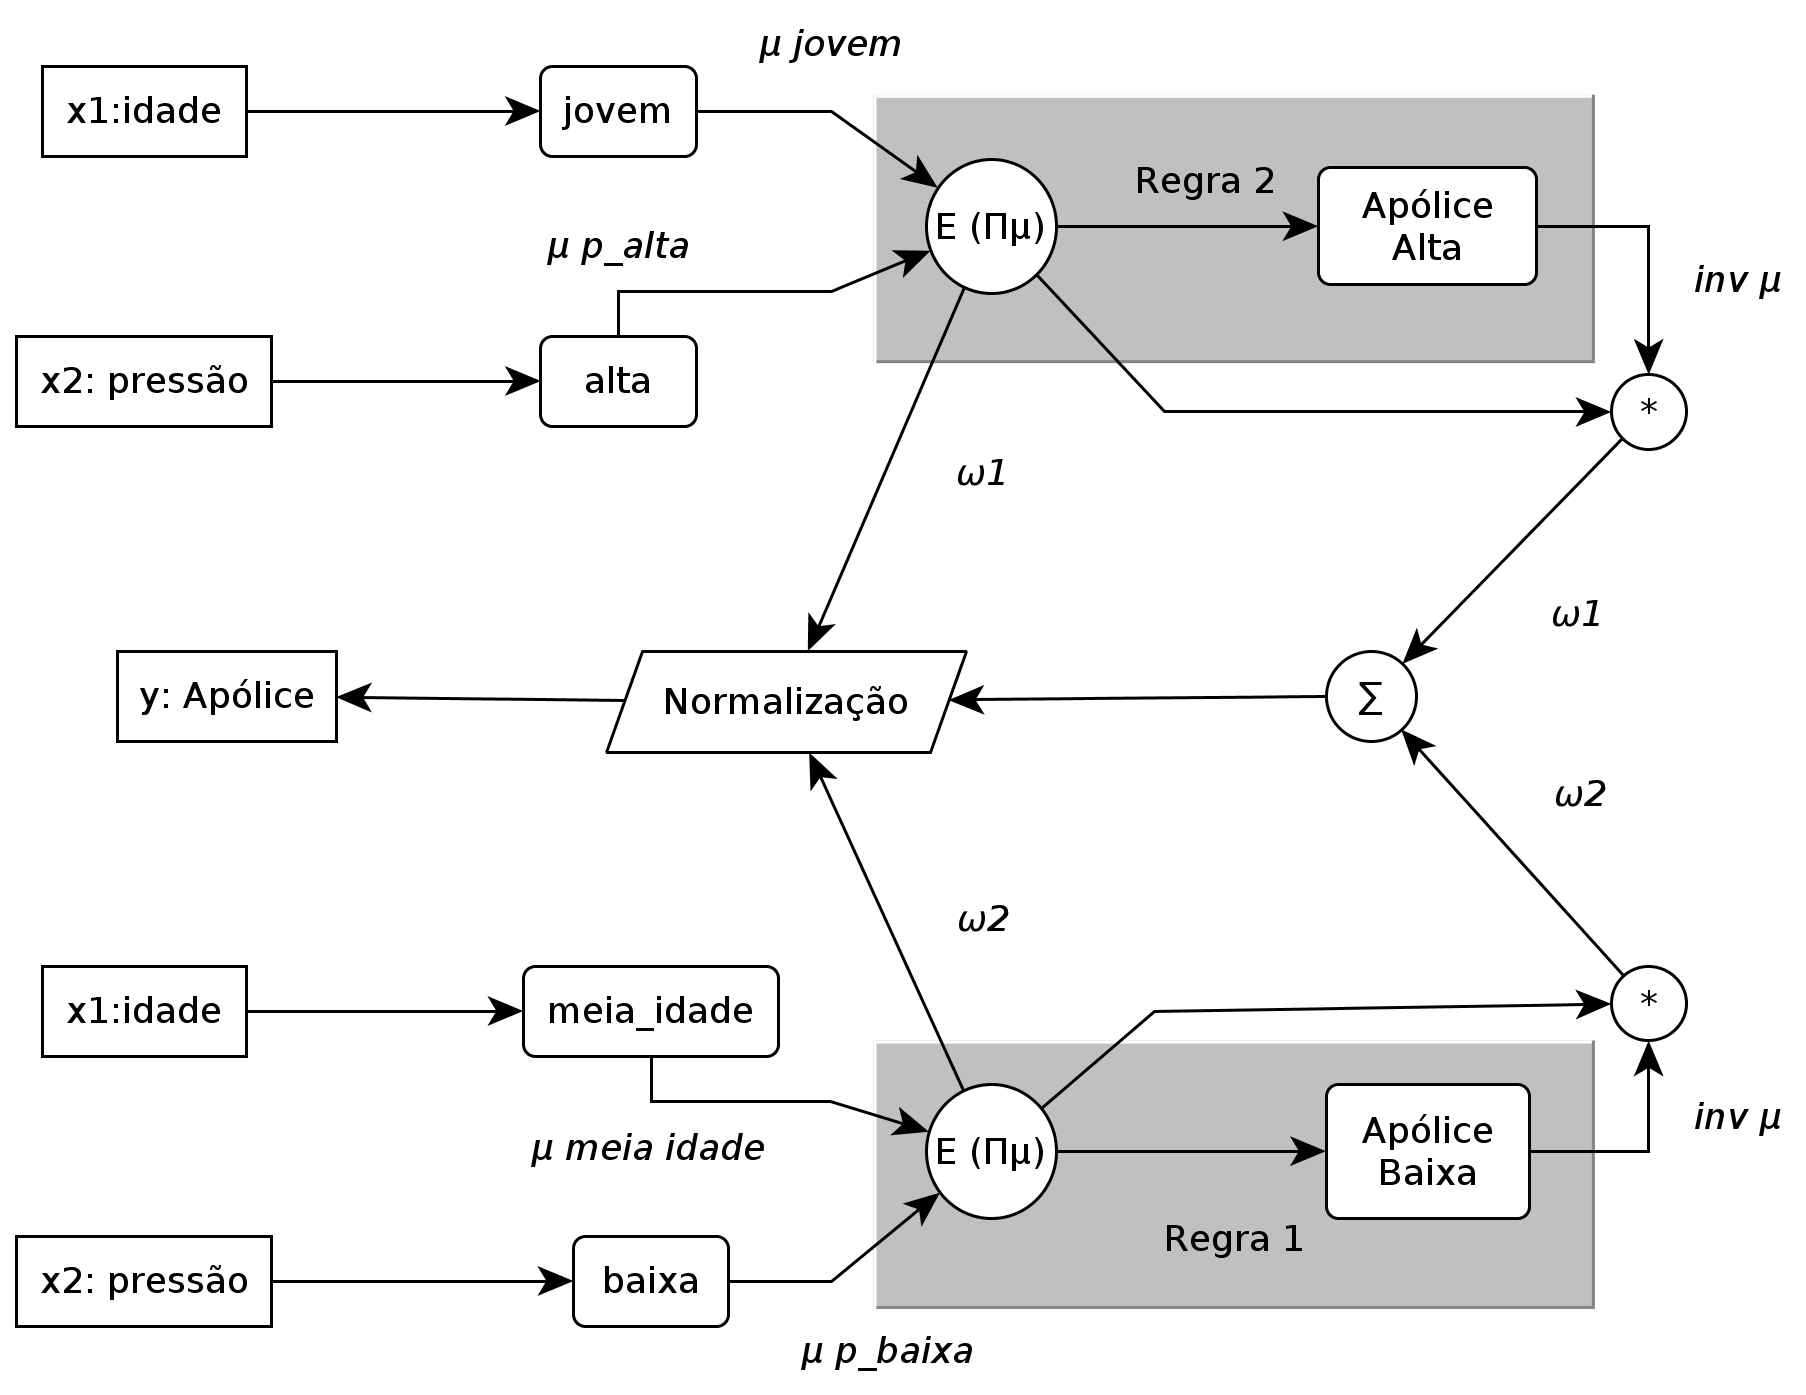
\includegraphics[width =0.6 \linewidth]
      {imgs/ex_logica_fuzzy}
      \caption{Exemplo de Aplicação}
    \end{figure}
  \end{block}
}

\frame{
  \frametitle{Lógica Nebulosa (SAM)}
  \begin{block}{}
    $$
    F(x) = \frac{\sum w_i.a_i(x).V_i.c_i}{\sum w_j.a_j(x).V_j}
    $$

    Com o volume/área $V_j$ e o centroide $c_j$ são dados por:

    $$
    V_j = \int{b_j(y_1, \cdots ,y_p)}_{\Re^{p}}.dy_1
    \cdots dy_p > 0
    $$

    $$
    c_j = \frac{\int{y.b_j(y_1,\cdots,y_p)}_{\Re^{p}}
    .dy_1 \cdots dy_p}{V_j}
    $$
  \end{block}
}

\section{Otimização da Colônia de Formigas}

Na busca por alimento, as formigas utilizam de feromônios para encontrar o melhor caminho.
Isso acontece da seguinte maneira: cada formiga deposita feromônio ao se deslocar. A partir
da avaliação da quantidade de feromônio depositada por formigas que já passaram pelo local,
formigas subsequentes tem mais probabilidade de se mover em rotas que tem mais feromônios. Ao
decorrer do tempo os feromônios vão evaporando, apagando rastros que não foram reforçados. 
Com isso, caminhos que são percorridos por mais formigas tem mais chance de serem 
percorridos por outras formigas do que aqueles que foram percorridos por menos formigas e 
caminhos que foram percorridos há pouco tempo tem mais chance de serem percorridos que caminhos
percorridos a muito tempo. A quantidade de feromônio depositado é mais intensa no trajeto de volta,
quando a comida foi encontrada. Outro fator que é levado em consideração é a qualidade da comida
encontrada, de maneira que mais feromônio é depositado quanto melhor for a fonte de alimento encontrada.
A medida que mais formigas exploram o local e encontram alimento, esse procedimento tende a otimizar o
trajeto entre a fonte de alimento e a colônia.

Apesar dessa heurística utilizada pelas formigas ser interessante para se resolver problemas combinatórios 
do tipo NP (i.e., com complexidade não polinomial), são necessárias algumas adaptações na construção
de um algoritmo computacional.

A seguir é apresentado a meta-heurística do algoritmo ACO (\textit{Ant Colony Optimization}),
juntamente com observações relacionadas as diferenças entre a heurística do ACO e o
comportamento natural das formigas descrito anteriormente.

\subsection{Meta-heurística do ACO}

\begin{figure}[ht]
  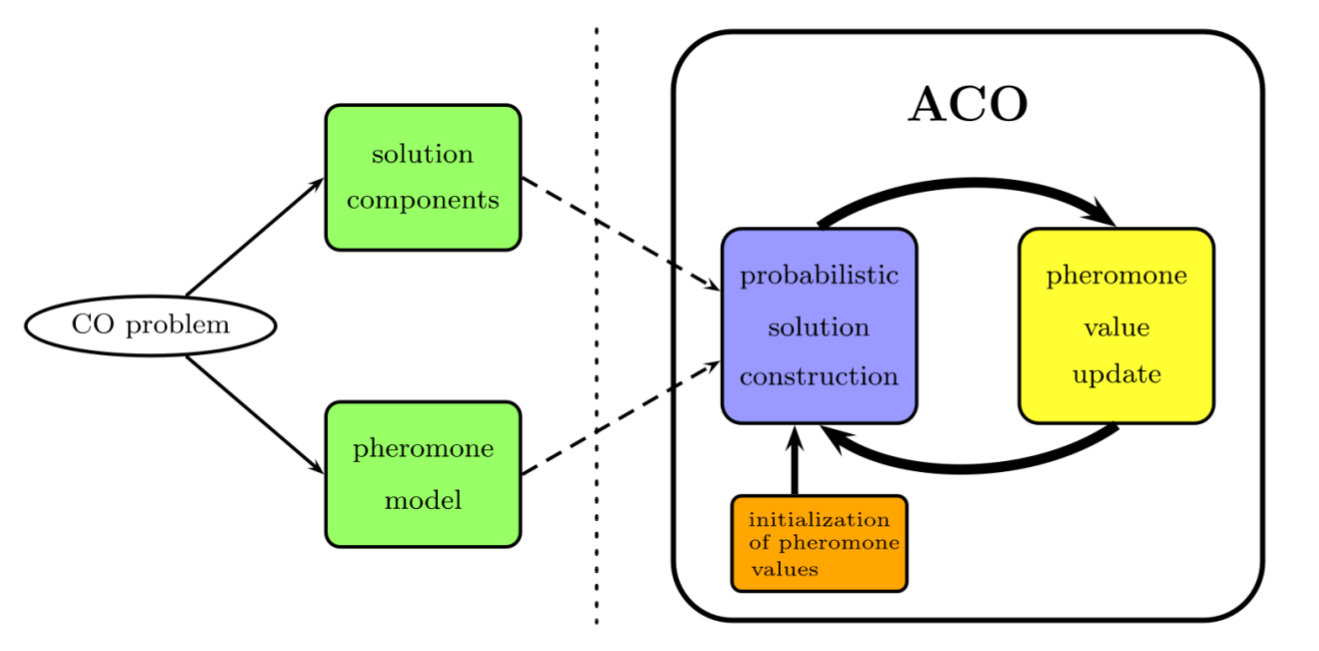
\includegraphics[width = 0.9 \linewidth]{imgs/meta_heuristica_aco}
  \caption{Diagrama de funcionamento da meta-heurística do ACO \cite{blum2005aco}}
  \label{diagrama_metaheuristica_aco}
\end{figure}

%Algoritmo
\begin{algorithm}[H]
  %Macros
  \SetKwBlock{AgendarAtividade}{AgendarAtividade}{fim}
  \SetKwBlock{Procedimento}{Procedimento}{fim}

  \Procedimento{
    \Enqto{$n < N_{MAX\_IT}$}{
      %\tcp*[f]{$N_{MAX\_IT}$ é o número máximo de iterações\\}
      \AgendarAtividade{
        ConstruirSolucoesFormigas\\
        AtualizarFeromonios\\
        %\tcp*[f]{opcional}\\
        \tcp{opcional:}
        AcoesGlobais
      }
    }
  }

  \caption{Pseudo código da meta-heurística do ACO\label{lst:meta-heuristica_aco}}
\end{algorithm}

A meta-heurística do ACO pode ser subdividida em três partes,
conforme proposto por \cite{doringo2004ant}: \textit{ConstruirSolucoesFormigas},
\textit{AtualizarFeromonios} e \textit{AcoesGlobais}.

\textit{ConstruirSolucoesFormigas} gerencia a movimentação de uma colônia de formigas
em torno dos nós vizinhos. A escolha do próximo nó é feita através de uma decisão
estocástica que é função da quantidade de feromônio no nós vizinhos e informação heurística.
Quando uma formiga encontra uma solução, ou enquanto a solução é construída, esta avalia a
qualidade da solução (completa ou parcial) que será utilizada pelo procedimento
\textit{AtualizarFeromonios} para decidir a quantidade de feromônio que será depositada.
Outro procedimento relevante na construção da solução é a eliminação de possíveis ciclos, utilizado
por exemplo, no problema do caixeiro viajante.

\textit{AtualizarFeromonios} é o processo que atualiza os traços de feromônio depositados pelas
formigas no espaço de busca. Os traços de feromônio podem aumentar, caso uma formiga tenha visitado
o nó/conexão em questão, ou diminuir, devido ao processo de evaporação do feromônio. Esse procedimento faz com 
que nós/conexões que foram visitados por muitas formigas ou por uma formiga e que tenha levado em
uma solução boa aumentem a probabilidade de serem visitados por futuras formigas. Semelhantemente, reduz 
a probabilidade de que nós que não foram visitados por novas formigas por muitas iterações sejam visitados
novamente. Logo, este procedimento evita a convergência a caminhos sub ótimos, favorecendo também a exploração
de novas regiões do espaço de busca.

Por fim, o procedimento \textit{AcoesGlobais} é utilizado para centralizar ações que não podem ser executadas
pelas formigas individualmente. Um exemplo de ações desse tipo é a filtragem de soluções ou o favorecimento de
regiões por meio de informações globais.

O procedimento \textit{AgendarAtividade} não necessariamente é uma instrução sequencial. Pode-se, portanto,
implementá-lo de maneira sequencial ou paralela, síncrona ou assincronamente. O tipo de abordagem que será
utilizada depende das características do problema que se deseja resolver.

\subsection{Exemplo de Aplicação}

\begin{figure}[ht]
  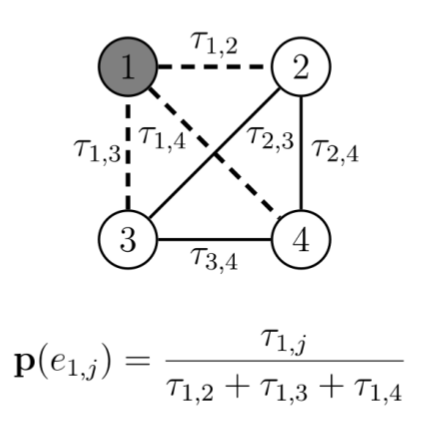
\includegraphics[width=0.32 \linewidth]{imgs/exemplo_aco_1}
  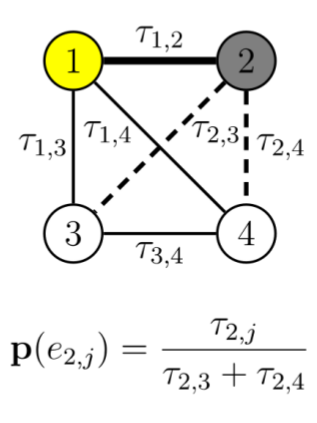
\includegraphics[width=0.32 \linewidth]{imgs/exemplo_aco_2}
  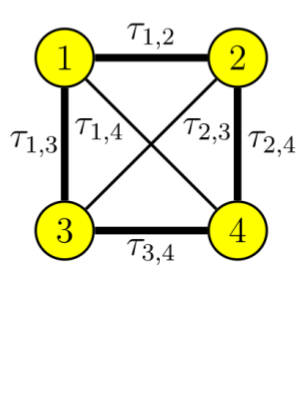
\includegraphics[width=0.32 \linewidth]{imgs/exemplo_aco_3}
  %\begin{subfigure}[b]
  %  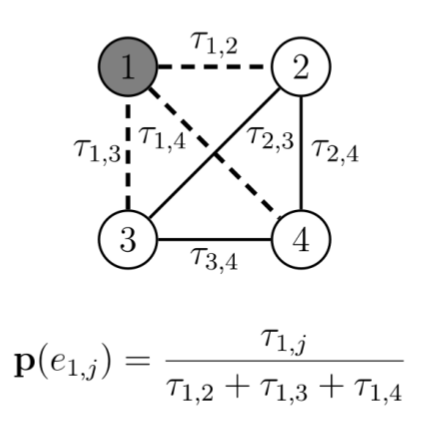
\includegraphics[width = 0.35 \linewidth]{imgs/exemplo_aco_1}
  %  \label{img:exemplo_aco_1}
  %\end{subfigure}
  %\begin{subfigure}
  %  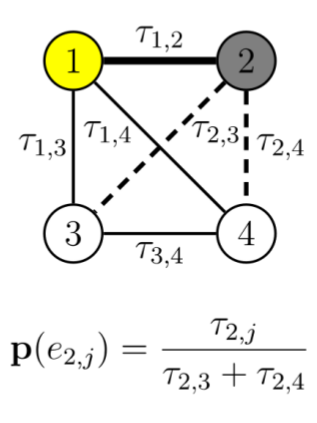
\includegraphics[width = 0.25 \linewidth]{imgs/exemplo_aco_2}
  %\end{subfigure}
  %\begin{subfigure}
  %  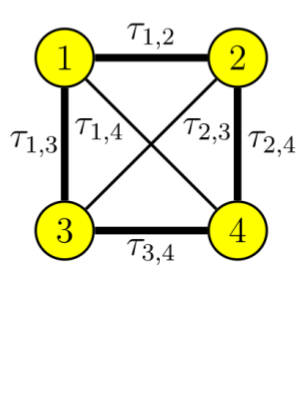
\includegraphics[width = 0.25 \linewidth]{imgs/exemplo_aco_3}
  %\end{subfigure}

  \caption{Example of the solution construction for a TSP problem}
  \label{img:exemp_aco}
  %It consists of 4 cities (modelled by a graph with 4 nodes; see Definition 1). The
  %solution construction starts by randomly choosing a start node for the ant;
  %in this case node 1. Figures (a) and (b) show the choices of the first,
  %respectively the second, construction step. Note that in both cases the
  %current node (i.e., location) of the ant is marked by dark gray color, and
  %the already visited nodes are marked by light gray color (respectively
  %yellow color, in the online version of this article). The choices of the ant
  %(i.e., the edges she may traverse) are marked by dashed lines. The probabilities
  %for the different choices (according to Eq. (4)) are given underneath the
  %graphics. Note that after the second construction step, in which we exemplary
  %assume the ant to have selected node 4, the ant can only move to node 3, and
  %then back to node 1 in order to close the tour. \cite{blum2005aco}}
\end{figure}

No TSP (\textit{Traveling Salesman Problem}) é dado um grafo completamente conectado e
não direcionado $G = (V , E)$ com pesos nas arestas.
Os nós $V$ do grafo representa as cidades e os pesos das arestas
distâncias entre as cidades. O objetivo é encontrar um caminho fechado em $G$
que contenha cada nó exatamente uma vez (portanto chamado passeio)
e cujo comprimento é mínimo. Logo, o espaço de busca $S$ consiste de todos os
passeios em $G$. O valor da função objetivo $f(s)$ de um passeio $s \in S$ 
é definido pela soma dos pesos das arestas que existem em $s$. O TSP pode ser
modelado de diversas maneiras como um problema de otimização discreta.
O modelo mais comum consiste de uma variável binária de decisão $X_e$ para
cada aresta em $G$.
Se em uma solução $X_e = 1$, então a aresta $e$ participa do passeio definido pela solução.

No que se refere abordagem do TSP usando ACO, 
as arestas de um dado grafo do TSP podem ser consideradas componentes da solução,
i.e., para cada $e_{i,j}$ é introduzido um valor de feromônio $\tau_{i,j}$. 
A tarefa de cada formiga consiste em construir uma solução plausível para o TSP, i.e.,
um passeio realizável. Em outras palavras, a noção de uma tarefa para uma formiga
muda de \textit{“escolher um caminho da colônia à fonte de comida”} para \textit{“
construir uma possível solução para o problema de otimização abordado"}. Note que com essa
mudança de tarefa, as noções de colônia e fonte de comida perdem seu significado.

Cada formiga constroem uma solução da seguinte maneira.
Primeiramente, um dos nós do grafo do TSP é aleatoriamente selecionada como sendo nó inicial.
Então, cada formiga constrói seu passeio no grafo do TSP movendo-se em cada iteração de construção
de seu nó atual (i.e., a cidade na qual ela esta localizada) á outro nó que ela ainda não visitou.
A cada passo (iteração) a aresta percorrida é adicionada a solução em construção. Quando não 
restam nenhum nó não visitado a formiga fecha o passeio movendo-se de seu nó atual até
o nó inicial, selecionado aleatoriamente no início da construção da solução. Dessa maneira a 
construção da solução implica que a formiga tem memória $T$ para armazenar os nó já
visitados. Cada iteração da solução é executado da seguinte maneira. 
Assumindo que a formiga esteja no nó $v_i$ , a subsequente iteração de solução é executada com probabilidade:

\begin{equation}
  \emph{p}(e_{i,j}) = \frac{\tau_{i,j}}{\sum_{k \in \lbrace 1,\dots,
  \vert V \vert\rbrace, v_k \not\in T}\tau_{i,k}},
  \forall j \in \lbrace 1,\dots,\vert V \vert\rbrace, v_j \not\in T
\end{equation}

Para um exemplo de tal construção de solução  veja Fig.~\ref{img:exemp_aco}.
Uma vez que todas as formigas de colônia tenham completado a construção de sua
solução, a evaporação do feromônio é executada da seguinte maneira:

\begin{equation}
  \tau_{i,j} \leftarrow (1-\rho)\cdot \tau_{i,j}, \forall \tau_{i,j}\in \mathcal{T}
\end{equation}

Onde $\mathcal{T }$ é o conjunto de todos os valores de feromônio.
Então as formigas executam seu respectivos passeios. Dessa maneira,
para cada $e_{i,j} \in s$ o seguinte feromônio é depositado:

\begin{equation}
  \tau_{i,j} \leftarrow \tau_{i,j} + \frac{Q}{f(s)}
\end{equation}

Onde $Q$ é uma constante positiva e $f(s)$ é o valor da função objetivo
da solução $s$. O sistema esta iterativamente aplicando $n_a$ 
formigas por iteração até que condição de parada
(e.g., o tempo limite) seja satisfeita.
Mesmo que o algoritmo descrito acima tenha provado que o comportamento das formigas
descrito anteriormente (no inicio da seção) pode ser transferido para um algoritmo 
de otimização discreta, foi em geral descoberto que ele é inferior aos algoritmos do estado da arte
para a solução do TSP\@. Portanto, ao longo dos anos várias extensões e aprimoramentos do algoritmo
original de resolução do TSP usando ACO foram introduzidas. Todos eles cobrem a definição de
meta-heurística do ACO,
descrito anteriormente.

\section{Recozimento Simulado}

No processo de recozimento de um metal, a quantidade de energia interna livre esta intrinsecamente
relacionada ao processo de resfriamento em que o metal é submetido. Quanto mais rápido se
resfriam um metal mais energia é armazenada internamente. Isso pode ser explicado considerando que
o tempo que a estrutura leva para atingir o estado de menor energia é maior que o disponível devido
a redução da mobilidade dos átomos com o decaimento da temperatura. Com efeito, quanto maior a taxa de
resfriamento maior o número de defeitos na estrutura do sólido e menor o tamanho médio dos grãos.
Quando se reduz a taxa de resfriamento, há uma maior chance de se atingir configurações mais estáveis.
Como resultado, a energia interna é reduzida. De acordo com \cite{bertsimas1993simulated},
pode-se modelar a probabilidade $p_{ij}$ de uma configuração atômica $\{r_i\}$ com energia $E\{r_i\}$
passar para a configuração $\{r_j\}$ com energia $E\{r_j\}$ na temperatura $T$ como:

\begin{equation}
\mbox{$p_{ij}$}=\left\{
	\begin{array}{rl}
	1 & \mbox{se $E\{r_j\} \le E\{r_i\}$} \\
	exp\left\{-\frac{(E\{r_j\}-E\{r_i\})}{k_B.T}\right\} & \mbox{se $E\{r_j\} > E\{r_i\}$}
\end{array} \right.
\end{equation}

Onde $k_B$ é a constante de Boltzmann. Para se reduzir a energia livre, é necessário que uma
rotina de resfriamento seja escolhida de acordo com o tipo de material a ser resfriado.

Conforme proposto por Kirikpartrick, Gellett e Vechin (1983) e Cerny (1985), pode-se desenvolver
uma heurística probabilística para se encontrar o mínimo global de uma função custo que possua
vários mínimos locais fazendo-se uma analogia com o fenômeno físico descrito acima. A meta-heurística
induzida por este processo é chamada de meta-heurística \textit{Simulated Annealing}(Recozimento
Simulado), ou SA, apresentado a seguir.

\subsection{Meta-heurística do SA}

De acordo com \cite{bertsimas1993simulated}, os elementos básicos da meta-heurística do SA
para a resolução de um problema combinatório são:

\begin{enumerate}
 \item Um conjunto finito $S$.
 \item Um função custo $J$ de imagem real definida em $S$. Seja $S^* \subset S$ o conjunto de todos os mínimos globais da
 função $J$, suposto subconjunto próprio.
 \item Para cada $i \in S$ um conjunto $S(i) \subset S - \{i\}$, chamado de conjunto das vizinhos de $i$.
 \item Para cada $i$, uma coleção de coeficientes positivos $q_{ij}$, $j \in S(i)$, tal que $\sum_{j \in S(i)} q{ij} = 1$.
 \item Uma função não crescente $T: \textbf{N} \rightarrow (0,\infty)$, chamada de rotina de resfriamento. Aqui \textbf{N}
 representa o conjunto de inteiros positivos, e $T(t)$ é chamada de \textit{temperatura} no tempo $t$.
 \item Um estado inicial $x(0) \in S$.
\end{enumerate}

Com base na definições acima, tem-se o seguinte pseudo código para a meta-heurística do SA:

%Algoritmo
\begin{algorithm}[H]
%Macros
\SetKwBlock{Procedimento}{Procedimento}{fim}
\SetKwBlock{EscolherVizinho}{EscolherVizinho}{fim}
\SetKwBlock{CalcTransicao}{CalcTransicao}{fim}

\Procedimento{
  SetarValoresInicias\;
  \Para{$n = 1$ até $N_{MAX\_IT}$ ou $J(x^*) \le TOL$ }{
    \Para{$k = 1$ até $N_{MAX\_IT}$ ou a solução convergir}{
      \EscolherVizinho{
        selecionar algum $j \in S(i)$\;
      }

      \CalcTransicao{
        $\Delta J \leftarrow J(j)-J(i)$\;
        \Se{$Delta J \le 0$}{
          $x(t+1) \leftarrow j$\;
          $x^* \leftarrow j$\;
        }
        \Senao{
          %$q_{ij} \leftarrow exp^{\left\{-\frac{\Delta J}{T(t)} \rigth\}}$\;\\
          $q_{ij} \leftarrow exp^{ -\frac{\Delta J}{T(t)} } $\;
          \lSe{$random() < q_{ij}$}{$x(t+1) \leftarrow j$}
          \lSenao{$x(t+1) \leftarrow i$}
        }
      }
    }
    AtualizarTemperetura\;
  }
}

\caption{Pseudo código da meta-heurística do SA\label{lst:meta-heuristica_sa}}
\end{algorithm}

No algorítimo~\ref{lst:meta-heuristica_sa}, o procedimento \textit{AtualizarTemperetura} executa a
rotina de resfriamento através da função $T(t)$ definida anteriormente. Já o procedimento
\textit{EscolherVisinho} escolhe aleatoriamente um dos elementos da vizinhança do vértice atual $i$.

\section{Algorítimo Genético}

Um \emph{algorítimo genético} é uma heurística de busca que procura
imitar a seleção natural que ocorre no processo evolucionário dos
organismos vivos.

Nessa heurística, uma população de soluções (também chamadas de
indivíduos ou fenótipos) para problemas de otimização é evoluída para
conseguir soluções melhores. Cada solução possui um conjunto de
propriedades (cromossomos ou genótipos) que podem ser mutados ou
alterados.

Os requerimentos são, tipicamente:

\begin{itemize}
\item
  uma representação genética da solução
\item
  uma função de aptidão para avaliação da solução
\end{itemize}

\subsection{O processo}

O processo é iniciado com uma população com propriedades geradas
aleatoriamente.

A iteração da heurística se da em 3 etapas:

\begin{itemize}
\item
  procriação: indivíduos são pareados e é aplicada a operação de
  cruzamento (\emph{crossover})
\item
  mutação: alguns indivíduos são selecionados e é aplicada a operação de
  mutação (\emph{mutation})
\item
  seleção: é usada a função de aptidão para descartar os indivíduos
  menos aptos restando as soluções que de fato trouxeram alguma melhora.
\end{itemize}

As condições mais comuns para terminação do processo são as seguintes:

\begin{itemize}
\item
  encontrada uma solução que atende os requisitos mínimos
\item
  número fixo de gerações alcançado
\item
  recursos alocados (tempo ou dinheiro) alcançados
\item
  a melhor solução alcançou um patamar estável em que mais iterações não
  produzem soluções melhores
\item
  inspeção manual
\end{itemize}

\subsection{Limitações}

As limitações mais comuns no emprego de um algorítimo genético são:

\begin{itemize}
\item
  Funções de avaliação computacionalmente caras tornam essa heurística
  ineficiente.
\item
  Não escala bem com a complexidade, isto é, quando o número de
  elementos expostos a mutação é grande o espaço de busca cresce
  exponencialmente. Por isso, na prática algorítimos genéticos são
  usados para, por exemplo, projetar uma hélice e não um motor.
\item
  A melhor solução é relativa às outras soluções, por isso o critério de
  parada não é muito claro em alguns problemas.
\item
  Em muitos problemas os algorítimos genéticos tendem a convergir para
  um ótimo local ou as vezes pontos arbitrários em vez do ótimo global.
\item
  É difícil aplicar algorítimos genéticos para conjunto de dados
  dinâmicos. Pois as soluções podem começar a convergir para um conjunto
  de dados que já não é mais válido.
\item
  Algorítimos genéticos não conseguem resolver eficientemente problemas
  em que a avaliação é binária (certo/errado), como em problemas de
  decisão. Nesse caso buscas aleatórias convergem tão rápido quanto essa
  heurística.
\item
  Para problemas mais específicos existem outras heurísticas que
  encontram a solução mais rapidamente.
\end{itemize}

\subsection{Pseudo código de um Algorítimo Genético}

%\begin{lstlisting}
\begin{algorithm}[H]
\SetKwBlock{Procedimento}{Procedimento}{fim}

%Algorithm: GA(n, \ki, \mu)
\Procedimento{
  %// Initialise generation 0:
  $k \leftarrow 0$\;
  $P_k \leftarrow $ população de n indivíduos escolhidos aleatoriamente\;
  %// EvaluatePk:
  %\Para{cada $i$ em $P_k$}
  %Compute fitness(i) for each i ∈ Pk;
  %Computar a $avaliacao(i)$ para cada $i$ em $P_k$\;
  %while fitness of fittest individual in Pk is not high enough;
  \Enqto{a $avaliacao(i)$ de cada $i$ em $P_k$ não for boa o suficiente}{
    %// Create generation k + 1:
    %// 1. Copy:
    %Select (1−χ)×n members ofPk and insert into Pk+1;
    Selecionar os $(1 - \chi) \times n$ membros com maior $avaliacao(i)$ de $P_k$ e inserir em $P_{k+1}$\;
    %// 2. Crossover:
    %Select χ×n members of Pk; pair them up; produce offspring; insert the offspring into Pk+1;
    Selecionar $\chi \times n$ membros de $P_k$, pareá-los e inserir a cria em $P_{k+1}$\;
    %// 3. Mutate:
    %Select µ×n members of Pk+1; invert a randomly-selected bit in each;
    Selecionar os $\mu \times n$ membros de $P_{k+1}$ com maior $avaliacao(i)$ e inverter um bit aleatório de cada membro\;
    %// Evaluate Pk+1:
    %Compute fitness(i) for each i ∈ Pk;
    %Computar a $avaliacao(i)$ para cada $i$ em $P_{k+1}$\;
    %// Increment:
    %k := k + 1;
    $k \leftarrow k + 1$\;
  }
%return the fittest individual from Pk;ut your code here.
  $melhor \leftarrow$ o membro $i$ em $P_k$ com maior $avaliacao(i)$\;
  \Retorna{$melhor$}
}
\end{algorithm}
%\end{lstlisting}

%\subsection{Referências}
%
%\begin{itemize}
%\item
%  \href{http://en.wikipedia.org/wiki/Genetic\_algorithm}{Genetic algorithm}
%\item
%  \href{http://www.cs.ucc.ie/~dgb/courses/tai/notes/handout12.pdf}{Genetic Algorithms - Derek Bridge}
%\end{itemize}

% TODO[jansegre]: exemplo de utilização
% TODO[jansegre]: como pode ser utilizado

\section{Rede Neural}

O termo mais apropriado é rede neural aritificial, já que apenas rede
neural pode se referir ao sistema biológico de nervos, no entando dado o
contexto desse texto e o uso consagrado do termo ``rede neural'', esse
será usado no lugar da versão mais explícita ``rede neural artificial''.

Uma rede neural é um sistema inspirado no sistema nervoso central (em
especial o cérebro) encontrado em muitos animais. A ideia básica é ter
um grafo em que cada nó abstrai um neurônio e é representado como uma
função, alguns desses nós são responsáveis pela observação e outros pela
saída e os nós de entrada alimentam os próximos nós até chegar nos nós
de saída. \cite{haykin2001redes}

\begin{figure}[H]
  \centering
  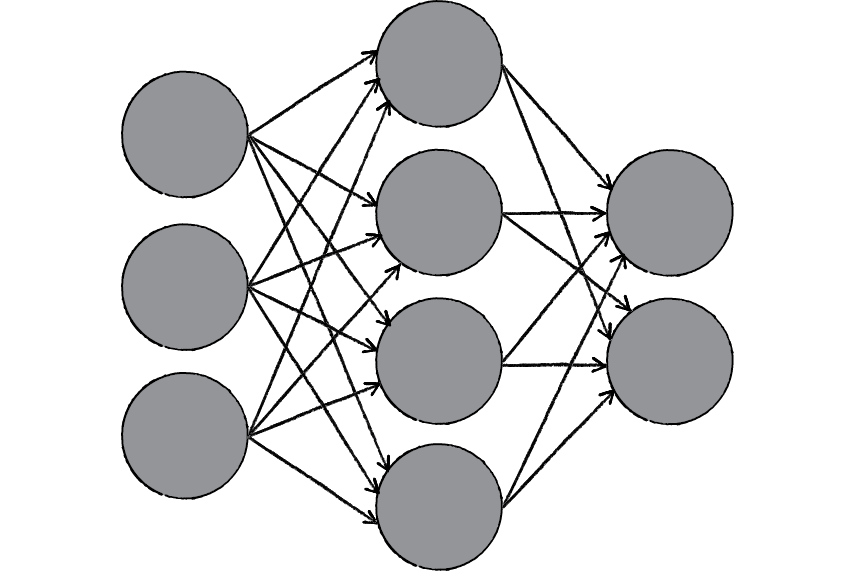
\includegraphics[width=10cm]{figuras/rede_neural_grafo}
  \caption{Rede neural com três camadas.}\label{fig:rede_neural_grafo}
\end{figure}

A figura \ref{fig:rede_neural_grafo} exemplifica uma rede neural \emph{feedforward},
que é baseada num grafo direcionado acíclico, em que podem ser vistas 3 camadas
a primeira é chamada de camada de entrada, a última, de saída e as intermediárias,
de escondidas. \cite{shiffman2012nature}

Um dos diferencias da rede neural é a capacidade de aprender, essa heurística
forma um sistem adaptativo. Existem três tipos de aprendizados:

\begin{itemize}
\item
  Aprendizado supervisionado: alimentar a rede com um problema cuja a solução é conhecida
  e depois fornecer a resposta certa para que a rede possa se ajustar.
\item
  Aprendizado não supervisionado: consiste em buscar padrões não conhecidos, não se conhece
  a resposta certa ou se uma resposta é certa ou não.
\item
  Aprendizado por reforço: alimentar a rede com um problema cuja a solução pode ser avaliada
  em boa ou má. Esse tipo de aprendizado é comum em robótica onde o robô caminha por um ambiente
  e tem o reforço negativo ou positivo de colodir ou encontrar o objetivo.
\end{itemize}

\subsection{O Neurônio}

O bloco de construção básico de uma rede neural são os neurônios.

\begin{figure}[H]
  \centering
  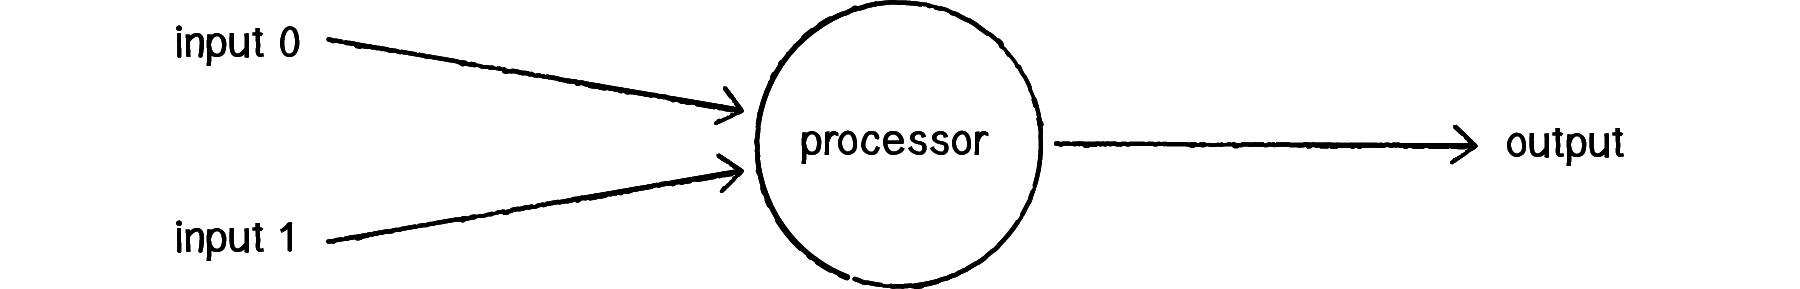
\includegraphics[width=10cm]{figuras/rede_neural_perceptron}
  \caption{Perceptron de duas entradas e uma saída.}\label{fig:rede_neural_perceptron}
\end{figure}

A figura~\ref{fig:rede_neural_perceptron} mostra um perceptron.

%\ldots{}

%\begin{itemize}
%\itemsep1pt\parskip0pt\parsep0pt
%\item
%  http://en.wikipedia.org/wiki/Neural\_network
%\item
%  http://en.wikipedia.org/wiki/Artificial\_neural\_network
%\item
%  HAYKIN, S. Redes neurais princípios e prática.
%\end{itemize}


% discussão da modelagem
\chapter{Análise das Possíveis Abordagens}\label{cap:anal_abordagens}

% TODO(depois): está muito obscuro, ligar com o final de cada heurística, não deve mudar muito esse capítulo.

\section{CRF}

Como os métodos AG (Algoritmo Genético), SA e ACO são heurísticas de otimização,
é necessário que o problema da aproximação de uma função seja reduzido a um problema
de otimização. A abordagem que se escolheu foi utilizar os \textit{conditional random
fields} para modelar um classificador para identificar as regras, ou táticas na
abstração da STP\@. Os métodos de otimização estudados anteriormente podem ser
aplicados para encontra os pesos do CRF.

\section{Lógica Fuzzy}

O método da Lógica Fuzzy, conforme exposto anteriormente, necessita que um conjunto
de regras seja definido. Essas regras poder ser geradas a partir de uma análise mais
detalhada do problema, mas também podem ser obtidas utilizando algum algorítimo de
aprendizagem de regras. Para aplicar esse método ao problema analisado neste trabalho
é necessário definir as regras e as distribuições das variáveis.

A vantagem dos conjuntos difusos é que eles tornam o modelo mais robusto. A lógica fuzzy
tenta melhorar a classificação e os sistemas de decisão.

A principal desvantagem deste método é a modelagem necessária para encaixar os conceitos
descritos acima. Isso, pois o conceito de conjuntos nebulosos ainda estão em desenvolvimento
para o problema abordado neste trabalho. Essa modelagem não é imediata, pois o problema é de
classificação temporal. Não basta que as características do ambiente sejam associadas aos
conjuntos nebulosos de características. É necessário que regras sejam especificadas estática
ou dinamicamente. No caso estático, elas seriam incorporadas ao modelo através de especialistas.
No caso dinâmico, uma solução é utilizar um classificador para deduzir as regras.

\section{Rede Neural}\label{cap:abordagem_rede_neural}

Essa abordagem consiste em usar uma Rede Neural que tem como entrada o estado do
jogo (todas as posições, orientações, velocidades e o comando do juiz) e como
saída o estado do time adversário (todas as posições, orientações e velocidades
dos robôs do time adversário), que visa prever as ações imediatas do adversário.
Essa rede deve ser treinada para prever um time específico usando os
\textit{logs} das partidas do torneio de 2013 da \textit{RoboCup}.

\subsection{Prova de conceito}

% TODO[jansegre] observação em <posição da bola>

Para prova de conceito, com o objetivo de estudar o pré-processamento
a ANN foi desenvolvido um programa para prever a
posição da bola. Foi implementado uma Rede Neural \textit{feedforward} com uma
camada oculta cujo
número de nós foi variado entre 8 e 320. Os nós de entrada foram 4: posições $x$
e $y$, e velocidades em $x$ e $y$, como os \textit{logs} não possuem informação
de velocidade essa foi calculada usando a diferença entre dois quadros
consecutivos. São 2 nós de saída: as posições $x$ e $y$, do próximo quadro. Foi
usada ativação sigmoid simétrica. Nessa implementação o treinamento convergiu
para um erro muito alto, como pode ser visto abaixo na saída (resumida) do
treinamento com 32 nós ocultos, é usado o erro médio quadrático e a unidade de
distância é o milímetro.

% saída do treinamento
\lstinputlisting{../train.log}

Esse problema não era esperado, foi decidido que seria necessário analisar
melhor os dados de treinamento para entender os motivos do ocorrido. Para tanto
foi modificada uma ferramenta desenvolvida no laboratório, originalmente usada
para visualizar as partidas em tempo real, a fim de visualizar os \textit{logs}
das partidas. Ao inspecionar esses logs notou-se dois tipos de irregularidades
relevantes para o treinamento, mostradas na figura~\ref{fig:logs}.

%\begin{figure}[thpb]
%  \centering
%  \begin{subfigure}[b]{0.49\textwidth}
%    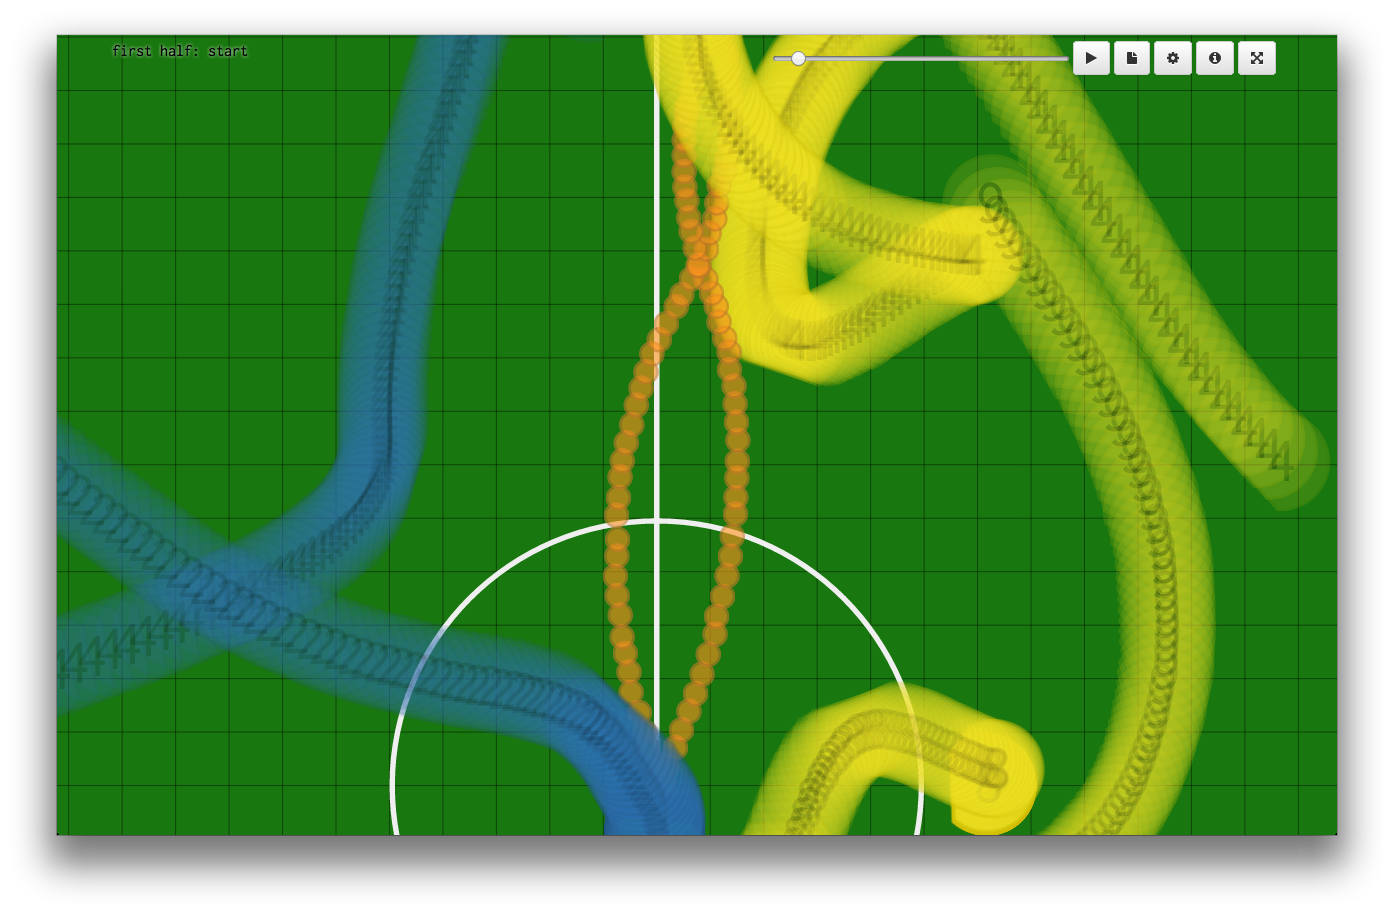
\includegraphics[width=\textwidth]{figuras/log_rastro.png}
%    \caption{Rastro duplo divergente}\label{fig:log_rastro}
%  \end{subfigure}
%  \begin{subfigure}[b]{0.49\textwidth}
%    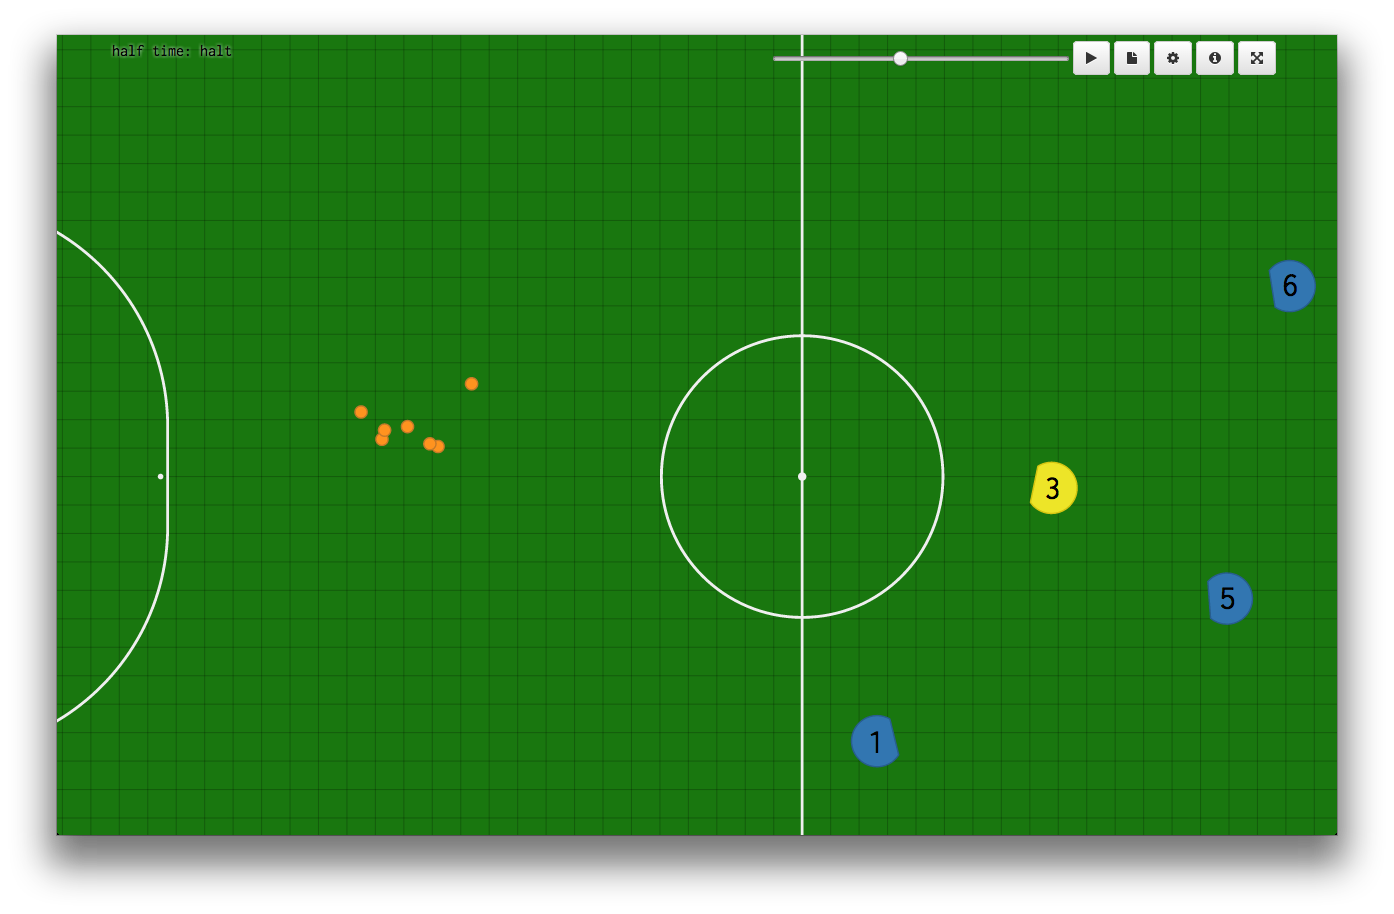
\includegraphics[width=\textwidth]{figuras/log_multi.png}
%    \caption{Objetos "fantasmas"}\label{fig:log_multi}
%  \end{subfigure}
%  \caption{Análise dos logs.}\label{fig:logs}
%\end{figure}

A figura~\ref{fig:log_rastro} mostra o problema que ocorre numa faixa no meio do
campo: a posição dos objetos (robôs e bola) oscila quadro a quadro. O motivo
desse problema é o fato das duas câmeras que capturam os dados possuírem uma
área de interseção e devido a diferenças sutis na calibração a posição dos
objetos difere quando vista de câmeras distintas. Uma saída trivial seria
ignorar os dados de uma das câmeras, mas isso é não é desejado pois uma parte
fundamental do estado do jogo estaria sendo ignorada.

Já na figura~\ref{fig:log_multi}, pode ser observado o segundo problema: há
momentos em que vários objetos "fantasmas" aparecem, isto é, são detectados
objetos que não existem no campo físico. O efeito disso é que a posição da bola
muda drasticamente para pontos que não fazem sentido.

A abordagem da rede neural, apesar de ocultar a semântica da relação dos fatores
analisados, parece bem apta a resolver o problema. Porém é necessário contornar
o problema dos dados de treinamento para poder implementar uma solução de fato.

% vim: tw=80 et ts=2 sw=2 sts=2



% próximas etapas
\section{Próximas Etapas}

As próximas etapas consistem em estudar a solução através dos métodos e das abordagens 
propostas de problemas mais simples para consolidar o estudo dos métodos estudados e 
analisar as topologias das redes neurais para que futuramente seja possível encontrar 
a topologia ótima e assim refinar os resultados da rede e das regras do sistema difuso.



% bibliografia
\section{Referências}
\frame{
\frametitle{Referências}
\begin{itemize}
\item SPONG, M. W.; VIDYSAGAR, M. \textbf{Robot Dynamics and Control}. Canadá. John Wiley and Sons: Singapore, 1989.
\item PIRES, Norberto J. \textbf{Robótica:} Das Máquinas Gregas à Moderna Robótica Industrial. Publicado no Jornal Público, caderno de computadores de 1 a 8 de julho de 2002.
\item CRAIG, John J. \textbf{Introduction to Robotics:} Machanics and Control. 3a ed. New Jersey: Pearson, 2005.
\item MARCHAND P., HOLLAND O. T. \textbf{Graphics and GUI's with MatLab}. 3a ed. New York: Chapman\&Hall/CRC,2003.
\end{itemize}
}
\frame{
\frametitle{Referências}
\begin{itemize}
\item BAXTER, Bill. \textbf{Fast Numerical Methods for Inverse Kinematics}. University of North Carolina at Chapell Hill: [s.n],2000. Disponível em http://billbaxter.com/courses/290/html/. Acesso em 02 de Novembro de 2012.
\item PAUL, Richard P.\textbf{Robot Manipulators:} Mathematics, Programming and Control. London: MIT Press, 1979.
\item ASADA A., SLOTINE J. J. \textbf{Robot Analysis and Control}. MIT: Jonh Wiley and Sons, [19--].
\item LEWIS, Frank, DAWSON, Darren M., ABDALLA, Chaouki T. \textbf{Robot Manipulator Control:} Theory and Practice. New York: Marcell Dekker,2004.
\end{itemize}
}
\frame{
\frametitle{Referências}
\begin{itemize}
\item BECKER, Marcelo. \textbf{Cinemática Inversa de Manipuladores Robóticos}.São Paulo: USP. Disponível em www.mecatronica.eesc.usp.br/wiki/upload/d/d6/Aula6.
\_SEM0317.pdf. Acesso em 07 de Setembro de 2012.
\item HERMINI, Helder A. \textbf{Robótica}.Campinas: UNICAMP. Disponível em www.fem.unicamp.br/~hermini/Robotica/Apresenta/aula3p1.pps. Acesso em 31 de Agosto de 2012.
\end{itemize} 
}
\frame{
\frametitle{Referências}
\begin{itemize}
\item SANTOS, Vitor M. F.\textbf{Robótica Industrial}. Departamento de Engenharia Mecânica: Universidade de Aveiro, [2003-2004]. Disponível em http://www2.mec.ua.pt/activities/disciplinas/RoboticaIndustrial /Apontamentos/v2003-2004/ RoboticaIndustrial-Sebenta2003-2004-v2a
.pdf. Acesso em 07 de Setembro de 2012.
\end{itemize} 
}


% pagina para assinaturas, deveria ser outro documento?
\newpage
%[Verificar se os nomes estão corretos inclusive a grafia]

\begin{center}
\_\_\_\_\_\_\_\_\_\_\_\_\_\_\_\_\_\_\_\_\_\_\_\_\_\_\_\_\_\_\_\_\_\_\_\_\_\_\_\_\_\_\_\_\_\_\_\_\_\_\_ \\
Jan Lucas de Lima Segre (10417) \\Aluno \\ 
\end{center}
\hspace{4cm}
\\

\begin{center}
\_\_\_\_\_\_\_\_\_\_\_\_\_\_\_\_\_\_\_\_\_\_\_\_\_\_\_\_\_\_\_\_\_\_\_\_\_\_\_\_\_\_\_\_\_\_\_\_\_\_\_ \\
Victor Bramigk (??) \\Aluno \\ 
\end{center}
\hspace{4cm}
\\


\begin{center}
\_\_\_\_\_\_\_\_\_\_\_\_\_\_\_\_\_\_\_\_\_\_\_\_\_\_\_\_\_\_\_\_\_\_\_\_\_\_\_\_\_\_\_\_\_\_\_\_\_\_\_ \\
Paulo F. F. Rosa, Ph.D \\Orientador \\ 
\end{center}
\hspace{4cm}
\\


%\_\_\_\_\_\_\_\_\_\_\_\_\_\_\_\_\_\_\_\_\_\_\_\_\_\_\_\_\_\_\_\_\_\_\_\_\_\_\_\_\_\_\_\_\_\_\_\_\_\_\_ \\
%Ten Cel Ronaldo Moreira Salles, Ph.D \\Coordenador de Pós-Graduação \\
%
%\hspace{4cm}
%
%\end{center}

%Concordo com a presente Proposta de Dissertação e declaro que as necessidades para sua execução serão garantidas pelo departamento.

%\begin{center}
%
%\_\_\_\_\_\_\_\_\_\_\_\_\_\_\_\_\_\_\_\_\_\_\_\_\_\_\_\_\_\_\_\_\_\_\_\_\_\_\_\_\_\_\_\_\_\_\_\_\_\_\_\_\_\_\_\_\_\_\_ 
%
%Ten Cel José Antônio de Sousa Fernandes \\
%CHEFE SE/8
%\end{center}

\begin{center}

IME, em \today
\end{center}

\hspace{4cm}

\end{document}

\end{document}
